%%%%%%%%%%%%%%%%%%%%%%%%%%%%%%%%%%%%%%%%%%%%%%%%%%
%  Chilpancingo de los Bravos, Guerrero, México  %
%         15 noviembre del 2022 23:20            %
%      Congreso de estudiantes de Posgrado       %
%        Universidad Autónoma de Guerrero        % 
%          Plantilla Desarrollada por:           %
%          M.Sc. Camilo Mora Batista             %
%             Profesor Asistente                 %
%         Universidad de Holguín, Cuba           %
%%%%%%%%%%%%%%%%%%%%%%%%%%%%%%%%%%%%%%%%%%%%%%%%%%
\documentclass[a4paper,12pt]{article}
\usepackage[margin = 2.5cm, top =2.4cm]{geometry}
\usepackage[spanish]{babel}
\usepackage{times}
\usepackage[T1]{fontenc}
\usepackage[utf8]{inputenc}
\usepackage{plain}
\usepackage{graphicx}
\usepackage{fancyhdr}
%\usepackage{chicago} %Descomentar aqui para cambiar a estilo chicafo en las bibliografias
%\usepackage{apacite} %Descomentar aqui para cambiar a estilo APA 6ed en las bibliografia  

\fancypagestyle{plain}{
	\fancyhead[L]{\hspace{-2.5cm}
\includegraphics[scale=0.7]{leftheader2.png}}
	\fancyhead[C]{\quad\quad\vspace{1.5cm}
\includegraphics[width=15cm]{centerlistheadaer.jpg}}
	\fancyhead[R]{\vspace{0.5cm}\hspace{1cm}
\includegraphics[scale=0.6]{rightheader2.jpg}\hspace{-6.7cm}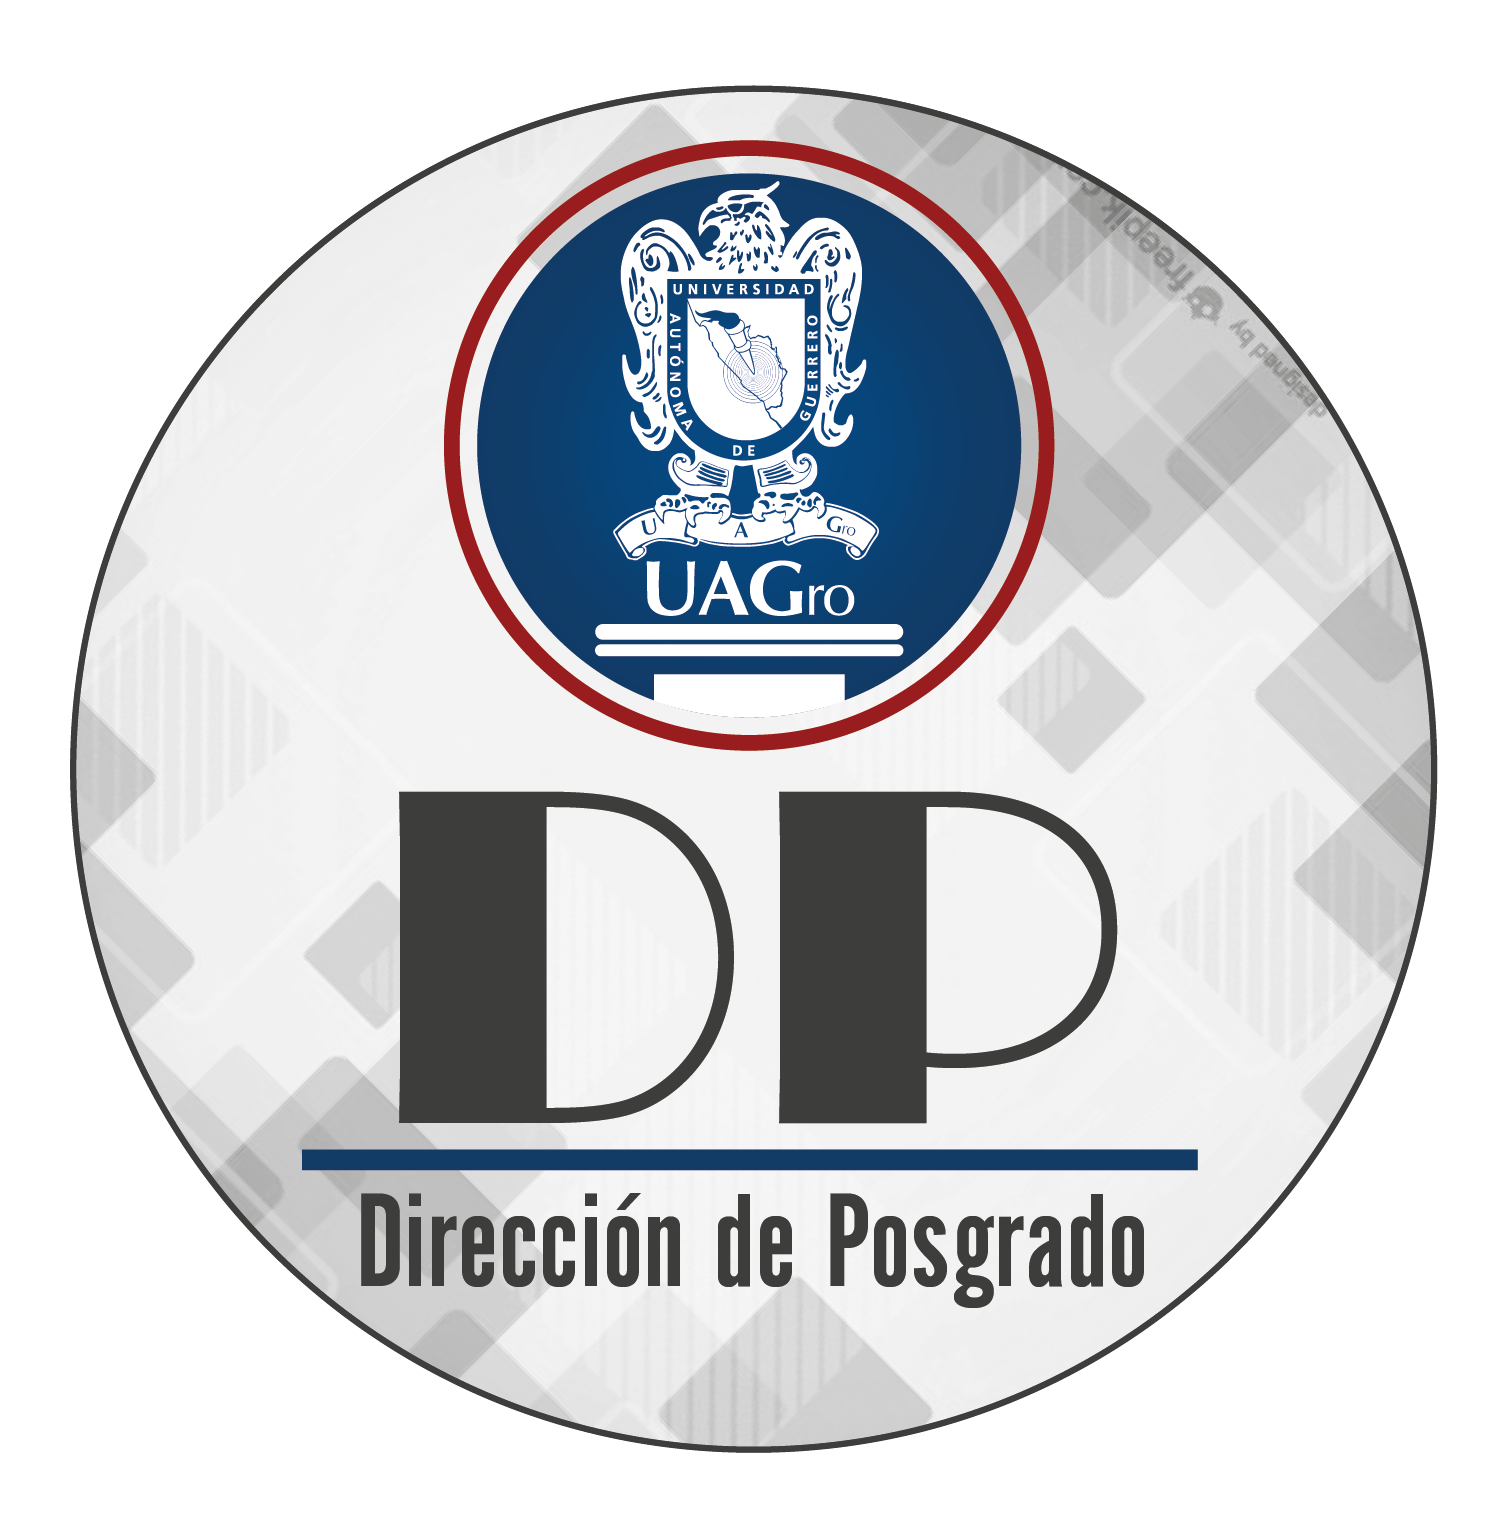
\includegraphics[scale=0.11]{rightheader1.png}\qquad\qquad\quad}
	%\fancyfoot[L]{L1}
	%\fancyfoot[C]{L2}
	%\fancyfoot[R]{L3}
	\renewcommand{\headrulewidth}{0pt}
	%\renewcommand{\footrulewidth}{0.5pt}
}



%\fancyhead[L]{\includegraphics{leftheader.png}}
%\fancyhead[C]{}
%\fancyhead[R]{\thepage}
\title{Revisión: Clasificación y predicción para el diagnóstico de las SCA2 a través de mediciones en Imágenes de Resonancia Magnética}

\author{José Alberto Cuesta$^1$,\underline{Camilo Mora Batista}$^2$, Cruz Vargas-de-Leon$^2$, \\ Maria Gúzman-Martínez$^2$, Frank Rodes-Carrillo$^1$, Sergio Torralbaz Fitz$^3$}

\date{}


\begin{document}
	%\vspace{-3in}
	\maketitle
	
	\begin{center}
		$ ^1$ Centro para la Investigación y Rehabilitación de las Ataxias Hereditarias, cuesta140560@gmail.com \\ 
		$^2$ Univerisdad Autónoma de Guerrero, narutokmy@gmail.com\\
		$^3$ Baptist Health South Florida. Biomedical Engineering department, torralbasfitz@gmail.com
	\end{center}
	
\section*{Resumen}
	
	La ataxia espinocerebelosa (SCA) es un término que hace referencia a un grupo de ataxias hereditarias, que son enfermedades neurológicas caracterizadas por la degeneración de las células que constituyen el cerebelo. A partir de los estudios que sugieren la Imagen por Resonancia Magnética (IRM) como un método importante que puede colaborar en el diagnóstico de las ataxias, se han investigado las mediciones lineales del Diámetro Antero-posterior del Mesencéfalo (ADM) en la IRM, correspondientes a estudios en pacientes SCA2 y Control. Para el desarrollo de la investigación se ha contado con la colaboración de 65 pacientes SCA2 y 39 pacientes Control siguiendo un criterio de inclusión y exclusión en ambos casos.  En esta ponencia se aborda una revisión sobre lo que se ha desarrollado en cuanto al diagnóstico de las atrofias en pacientes con SCA2 y la propuesta para enfrentar el problema científico identificado. También se resalta como puede aportar a los pacientes y en especifico a la investigación en Ataxias la predición y clasificación de los datos en IRM. 
	
	
\textbf{Palabras Clave:}  Ataxia Espinocerebelosa; Imagen de Resonancia Magnética; Diámetro Anteroposterior del Cerebro Medio
\section{Introductión}
	
	
El término ataxia, que no define una enfermedad o diagnóstico específico, se refiere a un estado patológico de la coordinación del movimiento \cite{luis_velazquez_perez_ataxia_2012,almaguer-gotay_spinocerebellar_2017,wilke_neurofilaments_2020} y se utiliza para describir un trastorno de la marcha que se manifiesta por inestabilidad incoordinación y aumento de la base de sustentación como consecuencia de una disfunción a nivel del cerebelo y/o de sus vías, así como de alteraciones en la médula espinal, los nervios periféricos o una alteración de estas tres condiciones \cite{almaguer-gotay_spinocerebellar_2017}.

De todas las formas de ataxias, las más comunes y por tanto las más estudiadas son las ataxias hereditarias.  Las ataxias hereditarias autosómicas dominantes son comúnmente conocidas como ataxias espinocerebelosas (SCA) \cite{mascalchi_neuroimaging_2020,rodriguez-labrada_founder_2020,prooije_spinocerebellar_2021}. Comprenden un amplio grupo de enfermedades neurodegenerativas caracterizadas por una gran heterogeneidad clínica, patoló-gica y molecular. En la actualidad se conocen 48 formas moleculares de SCA, aunque la heterogeneidad genética observada entre ellas sugiere que al menos el 30\% de su etiología molecular está por identificar \cite{luis_velazquez_perez_ataxia_2012}. \\
Las ataxias hereditarias son un grupo de enfermedades neurológicas heredi-tarias que afectan al cerebelo, la médula espinal, las vías espinocerebelosas y, normalmente, los nervios periféricos. Globalmente, se caracterizan por un síndrome atáxico con incoordinación motora central y de las extremidades \cite{paap_standardized_2016,assistance_publique_-_hopitaux_de_paris_identification_2019}. 
Se han realizado valiosas aportaciones que actualmente permiten conocer parte de las características genéticas de al menos 28 formas moleculares de Ataxias Espinocerebelosas Autosómicas Dominantes. De las 48 formas molecu-lares conocidas de Ataxia Espinocerebelosa ( SCA); la SCA2 representa el 15\% de todas las SCA a nivel internacional, y se distribuye en gran parte del mundo, sin embargo, en Cuba constituye el 76\% de las ataxias hereditarias \cite{meira_neuroradiological_2019,bhandari_spinocerebellar_2022}, específicas en la provincia de Holguín. \\
El diagnóstico de la ataxia espinocerebelosa cuenta con la ayuda de patólogos, radiólogos, neurólogos y genetistas. Los avances en el análisis y las pruebas genéticas moleculares agilizan la clasificación y el diagnóstico precoz definitivo. La determinación de un tipo específico de ataxia puede requerir tiempo y mucho apoyo económico. Por lo tanto, la manifestación clínica y la caracteriza-ción son imperativas antes del análisis genético. Pero los fenotipos de los distintos subtipos de SCA se solapan, por lo que el genotipo se ha convertido en el patrón de oro para el diagnóstico. Sin embargo, en los casos con características fenotípicas complejas o únicas, puede ser necesaria una evaluación genética adicional que guíe las pruebas genéticas específicas del subtipo definitivo \cite{silva_diagnosis_2019}.  En los subtipos más comunes y conocidos, como SCA1, SCA2, SCA3, SCA6, SCA7, SCA8 y SCA10, también se realizan análisis de sangre para detectar mutaciones. 



El diagnóstico de la SCA requiere un estudio costoso, lo que ha llevado a la búsqueda de biomarcadores más económicos. Esto ha llevado a la aparición de diferentes tipos de escalas de evaluación para descartar subtipos de ataxia. Entre estas escalas se encuentra la ICARS que fue la primera escala de ataxia y es ampliamente utilizada en estudios observacionales así como en ensayos de intervención \cite{bhandari_spinocerebellar_2022}. Consta de 19 ítems agrupados en cuatro subescalas que contribuyen a una puntuación total de 100 puntos \cite{paap_standardized_2016}. Las subdivisiones de los diferentes componentes de la ataxia son alteraciones posturales y de la marcha, ataxia de las extremidades, disartria y trastornos oculomotores. Otra de estas escalas clínicas es la SARA, basada en una evaluación semicuantitativa de la ataxia cerebelosa. Estas son las escalas más conocidas, pero existen otras escalas que se pueden encontrar en \cite{silva_diagnosis_2019,muthuswamy_diagnosis_2013}. También se encuentran estudios de registros electrooculográficos principalmente con casos de SCA2.

La neuroimagen permite evaluar las alteraciones morfológicas y funcionales del cerebro y la médula espinal en los pacientes con ataxia. La mayoría de los estudios de neuroimagen en la ataxia utilizan la resonancia magnética, pero también hay estudios de imagen molecular con radiotrazadores. En un reciente documento de consenso se analizó la aplicación de estos métodos de neuroimagen en la ataxia \cite{oz_mr_2020,klaes_mr_2016,wan_mr_2020}.  Las neuroimágenes demuestran la atrofia cerebelosa bruta más prominente en SCA2 y menos en otros subtipos, el agrandamiento de los ventrículos y la atrofia de otras partes del cerebro también \cite{cocozza_conventional_2021,cabeza-ruiz_convolutional_2021,cabeza-ruiz_convolutional_2022,klaes_mr_2016,oz_mr_2020,mascalchi_neuroimaging_2020}. 

En esta ponencia  se abordará el estado del arte del problema. Este consiste en conocer en que punto se encuentran las investigaciones de los pacientes con SCA2 desde las IRM, sus mediciones, y que técnicas matemáticas pueden aportar la invetigación. También se aborda los adelantos obtenidos en cuanto las lineas a trabajar para los resultados futuros. Mencionando la muestra que se ha obtenido para un posterior estudio en la clasificación y predicción de estos datos en estos pacientes.       
	
\section{Metodología}

En la ciudad de Holguín, Cuba existe un centro de investigación para estudiar los pacientes con ataxias hereditarias este nos ha permitido colaborar en sus investigaciones. Específicamente en el estudio de las imagénes obtenidas por Resonancia Magnética. Entre los hallazgos de este centro investigativo tiene como resultado que descubierto el inicio de la enfermedad SCA2 pueden mejorar la calidad de vida del paciente extendiéndola por un periodo mayor a los 5 años \cite{luis_velazquez_perez_ataxia_2012}. Por las características de la enfermedad no existe una cura ya que afecta el cerebelo tal es una zona muy delicada del cerebro primitivo. Esta región se encarga de controlar los movimientos de todo el cuerpo, por lo que al afectarse los movimientos  involuntarios del sistema respiratorio y digestivo es fatal para la vida del ser humano. En la Figura \ref{fig1} muestra regiones del cerebelo segmentadas semi-automaticas y el respectivo coeficiente R según la escala evaluativa de la progresión de la SCA2 \cite{klaes_mr_2016}.  

\begin{figure}[h]
 	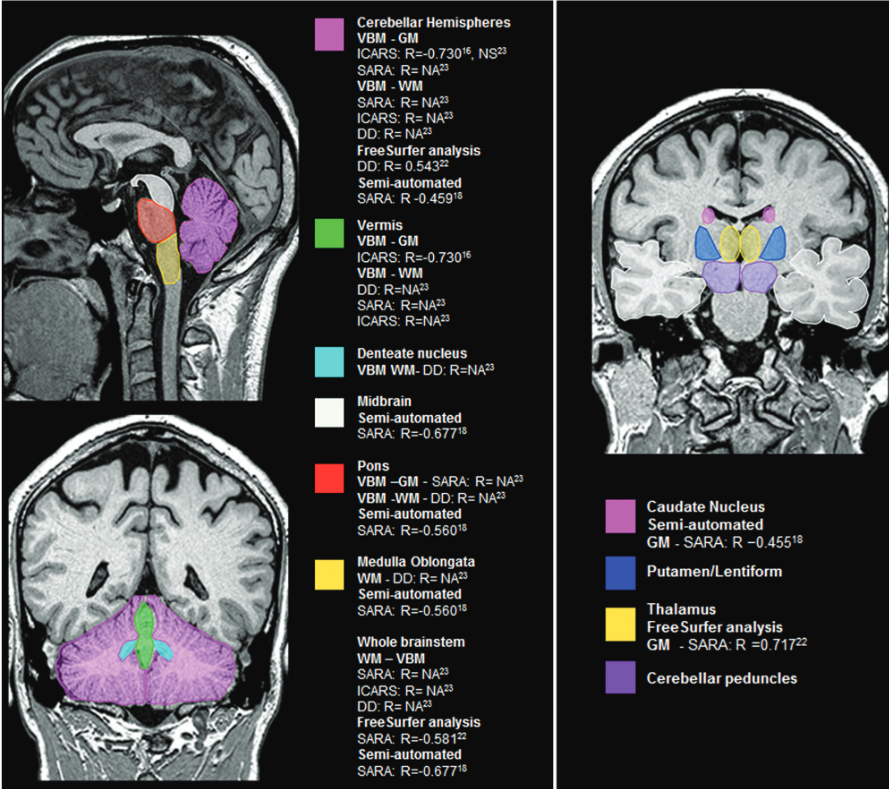
\includegraphics[scale=0.5]{resonanciamarcada.png}
 	\caption{IRM que muestra la region adectada en pacientes con SCA. Tomada de \cite{klaes_mr_2016}.}
 	\label{fig1}	
\end{figure} 

El estudio por IRM del cerebro en estos pacientes permiten detectar la atrofia en el cerebelo generada por esta enfermedad. Una vez medida la atrofia en las regiones que se afectan en el cerebelo, se puede valorar la progresión de la enfermedad. Hasta este momento no existe un biomarcador cuantitativo que permita evaluar la aparición de la SCA2 a partir de estudios por IRM. Esto se oborda con mayor rigurosidad en la discusión sección \ref{sec} de esta ponencia.                       



\subsection{Pacientes y Métodos}
Se realizó un estudio de casos y controles de precisión diagnóstica con pacientes y controles pertenecientes al Centro de Investigación y Rehabilitación de Ataxias Hereditarias Carlos Juan Finlay desde noviembre de 2020 hasta julio de 2022 en la provincia de Holguín. 


Los criterios de selección de los pacientes con SCA2 se mencionan a continuación. Criterios de inclusión: pacientes que presenten la mutación que causa la enfermedad SCA2. Dichos pacientes dieron su consentimiento para participar en el estudio. Criterios de exclusión: pacientes que presenten alguna enfermedad degenerativa, psiquiátrica, tumoral, tóxica, inmunomediada, metabólica o infecciosa que afecte al sistema nervioso. Los criterios de selección de los controles se mencionan a continuación. Criterios de inclusión: individuos que dieron su consentimiento informado para participar en el estudio. Criterios de exclusión: Individuos que presenten alguna enfermedad degenerativa, psiquiátrica, tumoral, tóxica, inmunomediada, metabólica o infecciosa que afecte al sistema nervioso.

\subsection{Procesamiento IRM}

Para el estudio de Resonancia Magnética Nuclear del cerebro, se utilizó el mismo protocolo de imágenes para los grupos SCA y Control.   El protocolo se realizó para esta investigación con un equipo Philips, modelo Panorama 0,23 T; con secuencias axiales, sagitales y coronales de T1, FFE 3D-24/90 con un espesor de corte de 5,5 mm siguiendo las líneas de referencia anatómicas establecidas. 

Se utilizó la herramienta Imagis 1.13 para obtener las mediciones de ADM. Las mediciones se realizaron manualmente, con parejas de expertos cegados, para garantizar la fiabilidad de las mediciones. Es importante destacar que los autores decidieron analizar la ADM porque la literatura investigada informa que en los pacientes con SCA2 la atrofia en el cerebelo es visible desde la RM. La ADM forma parte de esta área. De estos estudios se sabe que hay un aumento del espacio subaracnoideo. Esto es lo mismo que una disminución en la estructura del tronco cerebral, médula, cerebro medio \cite{reetz_brain_2018,jandeaux_biometry_2019,miranda_cerebellar_2022}.

La resonancia magnética estructural se ha utilizado para estudiar las alteraciones morfológicas cerebrales en pacientes con enfermedades neurodegenerativas, en particular en las SCA más comunes. La mayoría de los estudios se han centrado en la visualización y cuantificación de los cambios de volumen en el cerebelo y el tronco cerebral. Los diferentes tipos de SCA se caracterizan por rasgos clínicos específicos y superpuestos que requieren el estudio de sus genotipos. 

Los cambios morfológicos del cerebro asociados a diversos trastornos neurodegenerativos pueden estudiarse mejor {\em in vivo} con imágenes de resonancia magnética (IRM). Estudios anteriores en pacientes con SCA3/MJD han mostrado una estrecha correlación entre la atrofia del tronco cerebral y del cerebelo y las longitudes de las repeticiones de trinucleótidos CAG \cite{donath_neurofilament_2022}. Además, la atrofia del cerebelo y del tronco cerebral también se produce en SCA1, SCA2 y SCA7, y una atrofia cerebelosa significativa en SCA6 \cite{liang_correlation_2009,onodera_progressive_1998}.


Los estudios más recientes de neuroimagen en las SCA se centran en estudios volumétricos \cite{cabeza-ruiz_convolutional_2022}, en busca de un biomarcador que contribuya al diagnóstico precoz de la enfermedad, así como para estudiar la progresión \cite{coarelli_plasma_2021,mascalchi_neuroimaging_2020,straub_toward_2020}. 



En esta investigación utilizamos mediciones lineales obtenidas a partir de imágenes de resonancia magnética. Esto se debe a que la obtención de un estudio volumétrico con una resonancia magnética de 0,23 Tesla no es factible.  Sin embargo, sí permite estudiar las medidas lineales en cortes específicos. No es la primera vez que se estudian las mediciones lineales en la RM de pacientes con SCA.  Un estudio desarrollado por Xiaochun L. et al, utilizó mediciones lineales para estudiar la atrofia del cerebelo \cite{liang_correlation_2009}. En dicha propuesta utilizaron mediciones como: diámetros anteroposteriores del mesencéfalo, protuberancia y médula, diámetros superoinferiores del cuarto ventrículo y diámetros anteroposteriores y superoinferiores del cerebelo, fueron medidos en imágenes sagitales medias ponderadas en T1. La comparación categórica de los datos morfométricos entre los pacientes y los sujetos de control mostró un patrón de atrofia del cerebelo y de todo el tronco cerebral. Sin embargo, en particular el diámetro anteroposterior del cerebro medio fue significativamente diferente entre el grupo de control y el de SCA3 \cite{onodera_progressive_1998,liang_correlation_2009}.

Por este motivo, decidimos tomar el diámetro anteroposterior del mesencéfalo como variable para construir un modelo logístico que nos permitirá clasificar, predecir y contribuir al diagnóstico de la SCA2.

%\section{Resultado}



\section{Discución \label{sec}}

La resonancia magnética convencional forma parte del diagnóstico de las ataxias para confirmar la atrofia cerebelosa. Además, las tecnologías de RM cuantitativa se han utilizado para evaluar la estructura, la conectividad, la función y la bioquímica en las ataxias durante más de dos décadas \cite{oz_mr_2020,dogan_structural_2019,ashizawa_spinocerebellar_2018}. Ahora ha surgido una necesidad crítica de biomarcadores no invasivos y validados de la enfermedad cerebral y cerebelosa para facilitar los próximos ensayos clínicos en pacientes con SCAs y más específicamente SCA2 \cite{klockgether_spinocerebellar_2019}. 

La investigación de neuroimagen cuantitativa en las ataxias autosómicas recesivas se ha centrado en gran medida en la ataxia de Friedreich (FRDA) y las ataxias más comunes SCA1, SCA2, SCA3, SCA6, SCA7 . Esto se debe a que tener la posibilidad de contar con una gran muestra de datos es difícil debido a la baja tasa de prevalencia de las SCA. Hay artículos de este tipo que tienen una muestra pequeña y además muy variada en los diferentes tipos de SCAs \cite{j_alberto_cuesta_search_2022, faber_regional_2021,xie_quantitative_2020,brockmann_pet_2012,lindig_pattern_2019,li_neurofilament_2019}. Sin embargo, en el presente artículo toda la muestra estudiada pertenece a pacientes con SCA2 y puede contribuir al estudio cuantitativo de la atrofia en neuroimagen y, más concretamente, a la RM obtenida de pacientes con SCA2.   

En los últimos trabajos los trastornos más raros han sido a menudo objeto de informes cualitativos de casos, aunque hay varios estudios recientes de casos y controles \cite{selvadurai_multiple_2020,yang_lung_2022,yang_metabolic_2019,yap_magnetic_2022,rezende_developmental_2019}. En general, los estudios recientes de IRM no sólo han proporcionado una mejor delineación de los patrones de atrofia en las ataxias autosómicas recesivas y dominantes, sino que también se han alejado cada vez más de un enfoque miope de la macroestructura cerebelosa. 



\section{Conclusiones}

Este estudio ha permitido conocer el estado del arte en cuanto al tema de investigación. Debido a la baja tasa de prevalencia de esta enfermedad los artículos estudiados no han podido hacer un estudio riguroso para proponer un biomarcador basado en las mediciones de las IRM. La muestra construida para nuestro estudio es superior en cuanto a la muestra encontrada en los artículos estudiados. También es una muestra de solo un tipo de SCA, lo que nos permite proponer resultados cualitativos específicos de la SCA2.           




\bibliographystyle{plain} %usar {apacite} para APA 6d 
                          % usar {chicago} para Chicago style bibliography
\bibliography{refuagro}  

 
\end{document}